\documentclass[12pt,a4paper]{article}
\usepackage[T2A]{fontenc}
\usepackage[utf8]{inputenc}
\usepackage[russian]{babel}
\usepackage{amsmath}
\usepackage{amssymb}
\usepackage{graphicx}
\usepackage{floatrow}
\usepackage{booktabs}
\usepackage{wrapfig}
\usepackage{lipsum}
\usepackage{subcaption}
\usepackage{fancyhdr}

\newcommand{\figref}[1]{(См. рис. \ref{#1})}
\newcommand{\secref}[1]{(См. раздел. \ref{#1})}

\newcommand{\e}[1]{\text{$\cdot10^{#1}$}}

\pagestyle{fancy}
\fancyhead{}
\fancyhead[L]{Работа 2.1.3}
\fancyhead[R]{}
\fancyfoot[C]{\thepage}

\author{\normalsize Выполнил: Дедков Денис, группа Б01-109 \\
	\normalsize 21.04.2022}
\date{}

\usepackage{float}
\restylefloat{table}
\title{
	\large Отчет о выполнении лабораторной работы 2.1.3 \\
	\Large Определение $C_p/C_v$ по скорости звука в газе \\ 
	
}


\begin{document}
	\maketitle
	
\subsection*{Цель работы}
Измерение частоты колебаний и длины волны при резонансе звуковых колебаний в газе, заполняющем трубу.
Определение показателя адиабаты с помощью уравнения состояния идеального газа.

\subsection*{Оборудование и приборы} 
Звуковой генератор ГЗ;
электронный осциллограф ЭО;
микрофон;
телефон;
раздвижная труба;
теплоизолированная труба, обогреваемая водой из термостата;
баллон со сжатым углекислым газом;
газгольдер.
	
	
\subsection*{Теоретическое введение}

Cкорость распространения звуковой волны в газах зависит от показателя адиабаты $\gamma$.
На измерении скорости звука основан один из наиболее  точных методов определения показателя  адиабаты.

Скорость звука в газах определяется формулой:
$$c=\sqrt{\gamma\frac{RT}{\mu}},$$
где $R$ - газовая постоянная, $T$ - температура газа, а $\mu$ его молярная масса.
Выразим показатель адиабаты:
$$\gamma=\frac{\mu}{RT} c^2$$

Звуковая волна, распространяющаяся вдоль трубы, испытывает многократные отражения от торцов.
Звуковые колебания в трубе являются наложением всех отраженных волн и, вообще говоря, очень сложны.
Картина упрощается, если длина трубы L равна целому числу полуволн, то есть когда
$$L=n\frac{\lambda}{2},$$
где $\lambda$ — длина волны звука в трубе, а $n$ — любое целое число.

Скорость звука c связана с его частотой $f$ и длиной волны $\lambda$ соотношением:
$$c=\lambda f.$$

При постоянной длине трубы можно изменять частоту звуковых
колебаний.
В этом случае следует плавно изменять частоту $f$ звукового генератора, а следовательно, и длину звуковой волны $\lambda$.
Для $k$-ого резонанса получим:
$$L = (n+k)\frac{\lambda_{k+1}}{2}$$
$$f_{k+1} = \frac{c}{\lambda_{k+1}}=\frac{c}{2L}(n+k)=f_1 + \frac{c}{2L}k.$$

Скорость звука, деленная на $2L$, определяется, таким образом, по угловому коэффициенту графика зависимости частоты от номера резонанса.


\subsection*{Экспериментальная установка}

\begin{figure}[h]
	\caption{Схема установки}
	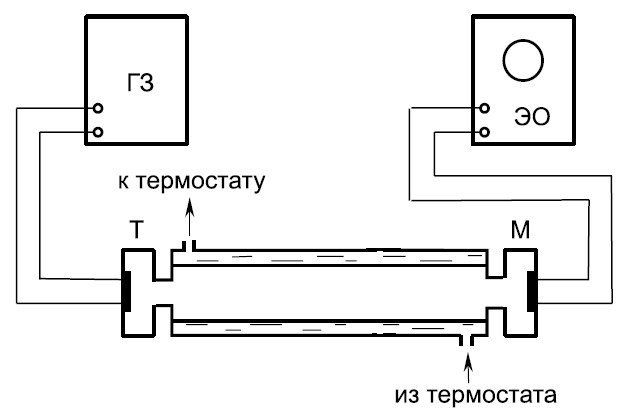
\includegraphics[scale=0.65]{res/scheme2.jpg}
	\label{scheme2}
\end{figure}

В установке звуковые колебания в трубе возбуждаются телефоном Т и улавливаются микрофоном М.
Мембрана телефона приводится в движение переменным током звуковой частоты; в качестве источника переменной ЭДС используется звуковой генератор ГЗ.
Возникающий в микрофоне сигнал наблюдается на осциллографе ЭО.

Микрофон и телефон присоединены к установке через тонкие резиновые трубки.
Такая связь достаточна для возбуждения и обнаружения звуковых колебаний в трубе и в то же время мало возмущает эти колебания: при расчетах оба торца трубы можно считать неподвижными, а влиянием соединительных отверстий пренебречь.

Установка \figref{scheme2} содержит теплоизолированную трубу постоянной длины.
Воздух в трубе нагревается водой из термостата.
Температура газа принимается равной температуре омывающей трубу воды.
На этой установке измеряется зависимость скорости звука от температуры.




\subsection*{Ход работы}
Проведём измерения $C_p/C_v$ для воздуха при различных температурах.
Для этого будем использовать трубу следующего постоянного размера:
$$L = (800 \pm 1) \text{ мм}.$$
Погрешность измерения температуры примем $\sigma_T = 0.5^\circ C$, несмотря на то, что прибор измеряет на порядок точнее. Связано это с тем, что температура, которую измеряет термостат может не полностью соответствовать температуре в трубке. 

Для фиксированной температуры будем изменять частоту звукового сигнала, тем самым изменяя и длину волны, так, чтобы мы могли наблюдать последовательные резонансы. Для каждого резонанса будем фиксировать частоту, при которой он возник. 

Данные занесем в таблицу \ref{tab:data}.

Перейдем к расчету зависимостей. Представим зависимость $f(k)$ в следующем виде:
$$F = f_{k+1} - f_1= \frac{c}{2L}k. = ax,$$
где обозначено $a = \frac{c}{2L}$.

Откуда легко заключить: зависимость $F(k)$ должна быть линейной.
Погрешность вычисления скорости звука и показателя адиабаты оценим с помощью закона накопления ошибок:


$$c \pm \sigma_c = 2La \cdot \left(1 \pm \sqrt{\varepsilon_L^2 + \varepsilon_a^2}\right),$$
$$\gamma \pm \sigma_\gamma=\frac{\mu}{RT} c^2 \left(1 \pm \sqrt{\varepsilon_T^2 + \left(2\cdot\varepsilon_c\right)^2}\right).$$


Статистическая обработка проведена \textbf{методом наименьших квадратов} и занесена в таблицу \ref{tab:mnk}.
Графики зависимостей $F(k)$ расположены на рисунке \ref{fig:fk}.

\begin{table}[H]
	\caption{Измерения частоты резонанса}
	\label{tab:data}
	\begin{tabular}{ccccccccc}
\toprule
$T,$ K & \multicolumn{2}{c}{295.8} & \multicolumn{2}{c}{301.0} & \multicolumn{2}{c}{311.0} & \multicolumn{2}{c}{321.0} \\
$k$ & $f$, Гц & $F$, Гц & $f$, Гц & $F$, Гц & $f$, Гц & $F$, Гц & $f$, Гц & $F$, Гц \\
\midrule
0 & 200 & 0 & 202 & 0 & 204 & 0 & 207 & 0 \\
1 & 450 & 250 & 453 & 251 & 460 & 256 & 466 & 259 \\
2 & 659 & 459 & 665 & 463 & 675 & 471 & 685 & 478 \\
3 & 872 & 672 & 880 & 678 & 894 & 690 & 907 & 700 \\
4 & 1087 & 887 & 1098 & 896 & 1115 & 911 & 1131 & 924 \\
5 & 1303 & 1103 & 1315 & 1113 & 1336 & 1132 & 1357 & 1150 \\
6 & 1519 & 1319 & 1533 & 1331 & 1557 & 1353 & 1582 & 1375 \\
7 & 1735 & 1535 & 1751 & 1549 & 1779 & 1575 & 1807 & 1600 \\
8 & 1951 & 1751 & 1969 & 1767 & 2000 & 1796 & 2031 & 1824 \\
9 & 2168 & 1968 & 2186 & 1984 & 2221 & 2017 & 2256 & 2049 \\
10 & 2384 & 2184 & 2405 & 2203 & 2443 & 2239 & 2481 & 2274 \\
11 & 2601 & 2401 & 2624 & 2422 & 2664 & 2460 & 2706 & 2499 \\
12 & 2817 & 2617 & 2841 & 2639 & 2887 & 2683 & 2932 & 2725 \\
13 & 3032 & 2832 & 3060 & 2858 & 3108 & 2904 & 3157 & 2950 \\
\bottomrule
\end{tabular}

\end{table}

\begin{figure}[H]
	\includegraphics[width = 11 cm]{c_sqrt_T.pdf}
	\caption{Зависимость $c(\sqrt{T})$ для воздуха}
	\label{fig:ct}
\end{figure}

		
\begin{figure}[H]
	\includegraphics[width = 14 cm]{F_k.pdf}
	\caption{Зависимость $F(k)$ для воздуха}
	\label{fig:fk}
\end{figure}

\begin{table}[H]
	\caption{Результаты вычислений для воздуха}
	\label{tab:mnk}
	\begin{tabular}{ccccccc}
\toprule
$T, \;$ K & $a, \; \text{c}^{-1}$ & $\sigma_a, \; \text{c}^{-1}$ & $c$, м/c & $\sigma_c$, м/с & $\gamma$ & $\sigma_{\gamma}$ \\
\midrule
295.8 & 216.44 & 0.48 & 346.3 & 0.9 & 1.414 & 0.008 \\
301.0 & 218.35 & 0.48 & 349.4 & 0.9 & 1.414 & 0.007 \\
311.0 & 221.84 & 0.50 & 354.9 & 0.9 & 1.413 & 0.008 \\
321.0 & 225.40 & 0.49 & 360.6 & 0.9 & 1.413 & 0.007 \\
\bottomrule
\end{tabular}

\end{table}



Усредняя по всем сериям получим:
$$	\langle\gamma\rangle = 1.413 \pm 0.004$$

Погрешность усредненного показателя адиабаты была оценена по следующей формуле:
$$\sigma_{\langle\gamma\rangle} = \frac{1}{n} \cdot \sqrt{\sum_{i = 1}^{n} \sigma_{\gamma_i}^2}$$

Построим также график скорости звука от корня из температуры $c(\sqrt{T})$, для качественной проверки теоретической зависимости (см. рис. \ref{fig:ct}).



\subsubsection*{Метод наименьших квадратов}
Метод наименьших квадратов в случае обработки линейной зависимости имеет следующий вид:

$$y = ax + b,$$

где $$a = \frac{r_{xy}}{ \sigma_x^2},$$
$$b = \overline{y} - a\overline{x}.$$

Для оценки погрешностей (стандартного отклонения) используем следующие формулы:
$$\sigma_a =  t_{n-1, p} \sqrt{\frac{1}{n-2} \left( \frac{\sigma_y^2}{\sigma_x^2} - A^2 \right)},$$
$$\sigma_b = \sigma_a \sqrt{\sigma_x^2 + \overline{x}^2},$$
где 
$n$ - количество измерений, $ t_{n-1, p}$ - коэффициент Стьюдента
Используя $a = \frac{c}{2L}$ получим значения $c$.
Рассчитаем $\gamma$ для каждой серии измерений.


\subsection*{Вывод}

В ходе работы изучили достаточно точный (погрешность порядка $1\%$) метод определения показателя адиабаты для воздуха. 

Результат, усредненный по четырем сериям имеет следующий вид:
$$	\langle\gamma\rangle = 1.413 \pm 0.004$$

\begin{description}
	\item[Применимость метода наименьших квадратов]
	Измеренные данные соответствуют критериям применимости метод наименьших квадратов. Погрешность отдельного измерения частоты резонанса мала ($~0.1\%$), а погрешности порядка (номера) резонанса нет. 
\end{description}

Имеет смысл указать некоторую особенность установки, которая может систематически повлиять на окончательную точность эксперимента:

\begin{description}
	\item[Измерение температуры.]
		Температура измерялась с помощью значения, которое показывал на табло термостат. Но эта температура может не совпадать с точным значением температуры в трубке. Для учета данной ошибки было принято решение взять погрешность измерения температуры порядка $0.5^\circ C$.
\end{description}
\end{document}